\documentclass[12pt]{article}
\usepackage[margin=1in]{geometry}
\usepackage{amsmath,amsthm,amssymb,amsfonts}
\usepackage{graphicx}

\newcommand{\N}{\mathbb{N}}
\newcommand{\Z}{\mathbb{Z}}

\newenvironment{part}[2][Part]{\begin{trivlist}
\item[\hskip \labelsep {\bfseries #1}\hskip \labelsep {\bfseries #2.}]}{\end{trivlist}}
%If you want to title your bold things something different just make another thing exactly like this but replace "problem" with the name of the thing you want, like theorem or lemma or whatever

\newenvironment{writeup}[2][Write-Up]{\begin{trivlist}
\item[\hskip \labelsep {\bfseries #1}\hskip \labelsep {\bfseries #2.}]}{\end{trivlist}}

\graphicspath{ {./} }


\begin{document}

%\renewcommand{\qedsymbol}{\filledbox}
%Good resources for looking up how to do stuff:
%Binary operators: http://www.access2science.com/latex/Binary.html
%General help: http://en.wikibooks.org/wiki/LaTeX/Mathematics
%Or just google stuff

\title{AST 540: Lab 1}
\author{Jonas Powell}
\maketitle

\begin{part}{}
  Describe the calibration procedure and record the system temperature that you measure along with the time at which you measured it. Collect data from the other observing groups and make two plots:

  \bigskip
  (1) system temperature as a function of time throughout the day \\
  \indent(2) system temperature as a function of ambient temperature.

  \bigskip
  By how much does the system temperature fluctuate throughout the day? Does it seem to track the ambient temperature? How does the system temperature compare to the theoretical quantum limit on the receiver temperature for this system?
\end{part}

\begin{writeup}{1}
  To calibrate our system, we began by moving the dish to a point on the sky at the same altitude as our source and slewed in azimuth until we were off any other radio sources and pressed the "Cal" button on the SRT GUI to get a cold sky measurement. We then sent Hunter outside to put the "absorber-on-a-stick" in front of the antenna's receiver, pressed "Enter" as prompted by the GUI, and allowed it to complete it's measurement. In this process, we found power values of:

  \begin{align*}
    P_{\text{cold}} &= 179.3 \\
    P_{\text{hot}} &= 358.7
  \end{align}

  We may then recall the Y-Factor calibration equations to solve for our receiver temperature.
  \begin{align*}
    y &= \frac{P_H}{P_C} \\
    T_{Rx} &= \frac{T_H - yT_C}{y - 1}
  \end{align}

  However, we obviously still need values of $T_H$ and $T_C$. We may extract these from the Johnson-Nyquist Noise Theorem:
  \begin{align*}
    T &= \frac{P}{kB}
  \end{align}
  where $B$ is the observation's bandwidth and $k$ is the Boltzmann constant.
\end{writeup}
\bigskip
\bigskip




\begin{part}{}
  Generate two plots of antenna temperature as a function of degrees offset in (1) azimuth and (2) elevation. Measure the HPBW of the SRT antenna in both azimuth and elevation. Are they the same? Why or why not? (Hint: Since the Sun is unlikely to be near the horizon, you will need to be careful with the azimuth axis. Try to figure out the appropriate correction factor to apply, since circles of constant elevation are not great circles.)
  \bigskip

  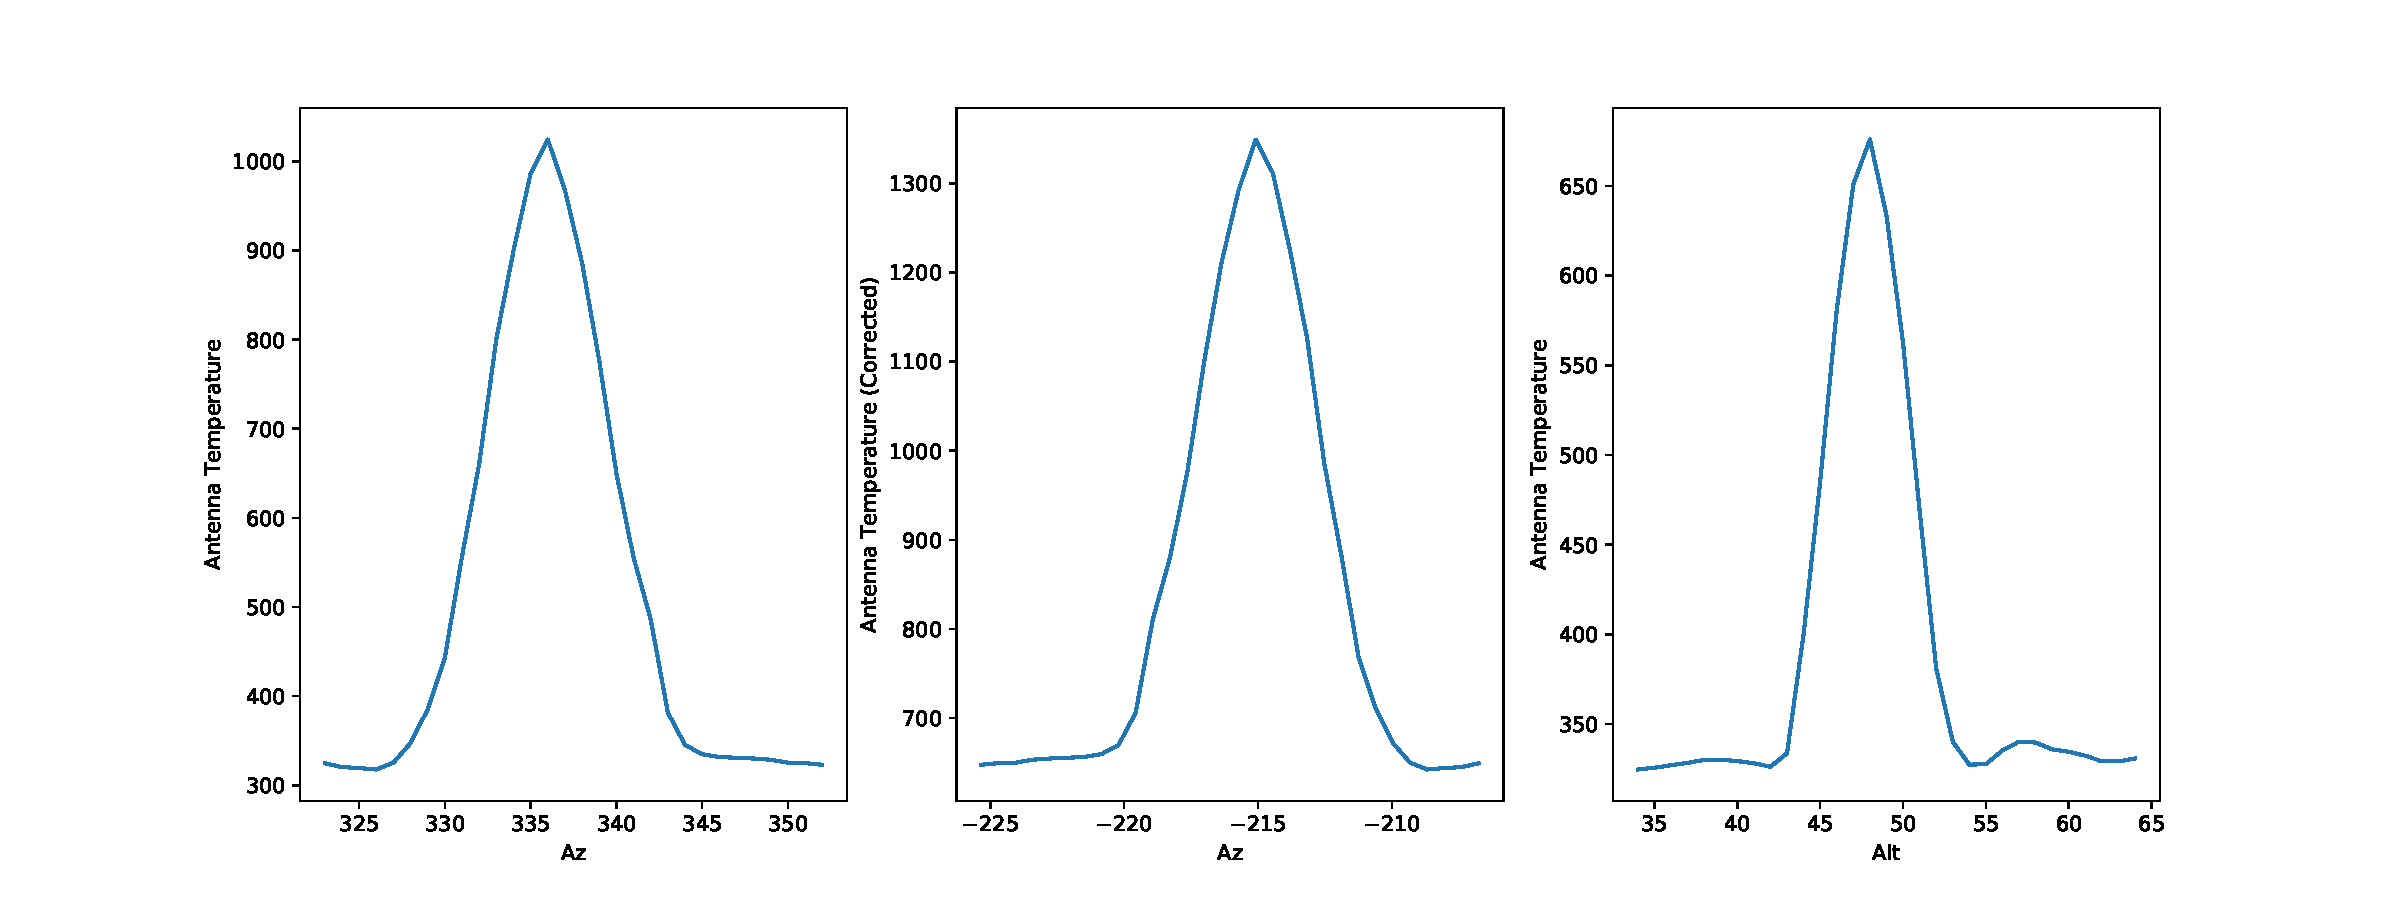
\includegraphics[scale=0.4]{part1} \\

  How does your plot of the gain pattern of the antenna compare with what you would expect for a uniform circular aperture (2.4m in diameter, observing at a wavelength of 21cm)? Plot an Airy function over your data (you will need to add a vertical offset to account for the system temperature). How does the beamwidth you measured compare with the theoretical expectation? Do you see the sidelobe levels you expected to see?
  \bigskip

  One reason your data will not match the theoretical expectation is that the aperture is undergoing nonuniform illumination (another reason is that the feed may be slightly out of focus). The tapered illumination caused by the beam pattern of the feed can be well approximated by the following function:
  \begin{align*}
    \epsilon(\rho) = [1 – (2\rho/D)^2]^{\gamma}
  \end{align}
  Which results in a gain pattern
  \begin{align*}
    G(\theta) = [2\gamma+1 (\gamma+1)!]^2 (4\pi A_g / \lambda^2) [J_{\gamma}+1(\pi D \theta/\lambda)/(\pi D \theta/\lambda)]^2
  \end{align}
  \bigskip

  For most real-life feeds, $\gamma \approx 1$. Try plotting the gain pattern for $\gamma = 1$, and see if it provides any improvement over the Airy pattern expected for the uniform illumination condition.
\end{part}

\begin{writeup}{1}

 blah
\end{writeup}


\bigskip
\bigskip

\begin{part}{}
  Calculate the aperture efficiency of the SRT, making sure to properly account for the system temperature. Look up the angular diameter of the Sun (cite your source) and use it along with your previous measurements of antenna temperature and aperture efficiency to estimate the flux density of the Sun at a wavelength of 21 cm. Collect your classmates’ measurements and plot the Solar flux as a function of time throughout the day (we might see a flare!).
  \bigskip

  Estimate the uncertainty on your measurement. Compare your measurement with the official NOAA record of Solar flux, which you can find on this web page:
  http://www.swpc.noaa.gov/ftpdir/lists/radio/7day_rad.txt
  \bigskip

  (Note: you will need to look up the Solar flux within 7 days of when you performed the experiment!) Using the NOAA records, estimate the spectral index of the Solar radiation. Is the spectrum thermal or nonthermal?
\end{part}

\begin{writeup}{1}

 blah
\end{writeup}


\end{document}
